\chapter{NMR in Depth: Pulses, Relaxation and 2D}\label{ch:b3:advanced-nmr}

A hospital MRI scanner and the NMR spectrometer of a chemistry department
work on the same principle. Each places hydrogen nuclei in a strong magnetic
field, tips their magnetisation with a short pulse of radio waves, and
listens to the faint signal it induces as it precesses and relaxes. The
scanner turns the signal into an image of soft tissue; the spectrometer into
a list of chemical shifts and couplings, and, with several pulses in a row,
into two-dimensional maps that show which atom is bonded to which. This
chapter explains what the pulses do, why the signal fades, and how
two-dimensional spectra are read --- the method by which most new organic
structures are now solved.

\begin{recall}
The Year 1 volume interpreted ${}^1$H NMR spectra: chemical shift, shielding,
equivalent protons, integration, spin--spin coupling, coupling constants and
multiplets. The Year 2 volume added ${}^{13}$C NMR with broadband decoupling and
DEPT, whose pulse sequence it took as given; the pulses are explained here.
\Cref{ch:b3:many-electron-atoms} treated spin as an angular momentum. From
physics: a magnetic moment in a field has energy $-\boldsymbol\mu\cdot\mathbf B$, and
populations of levels follow the Boltzmann factor $\eu^{-\Delta E/kT}$, developed
in \cref{ch:b3:partition-functions}.
\end{recall}

\begin{omfigure}
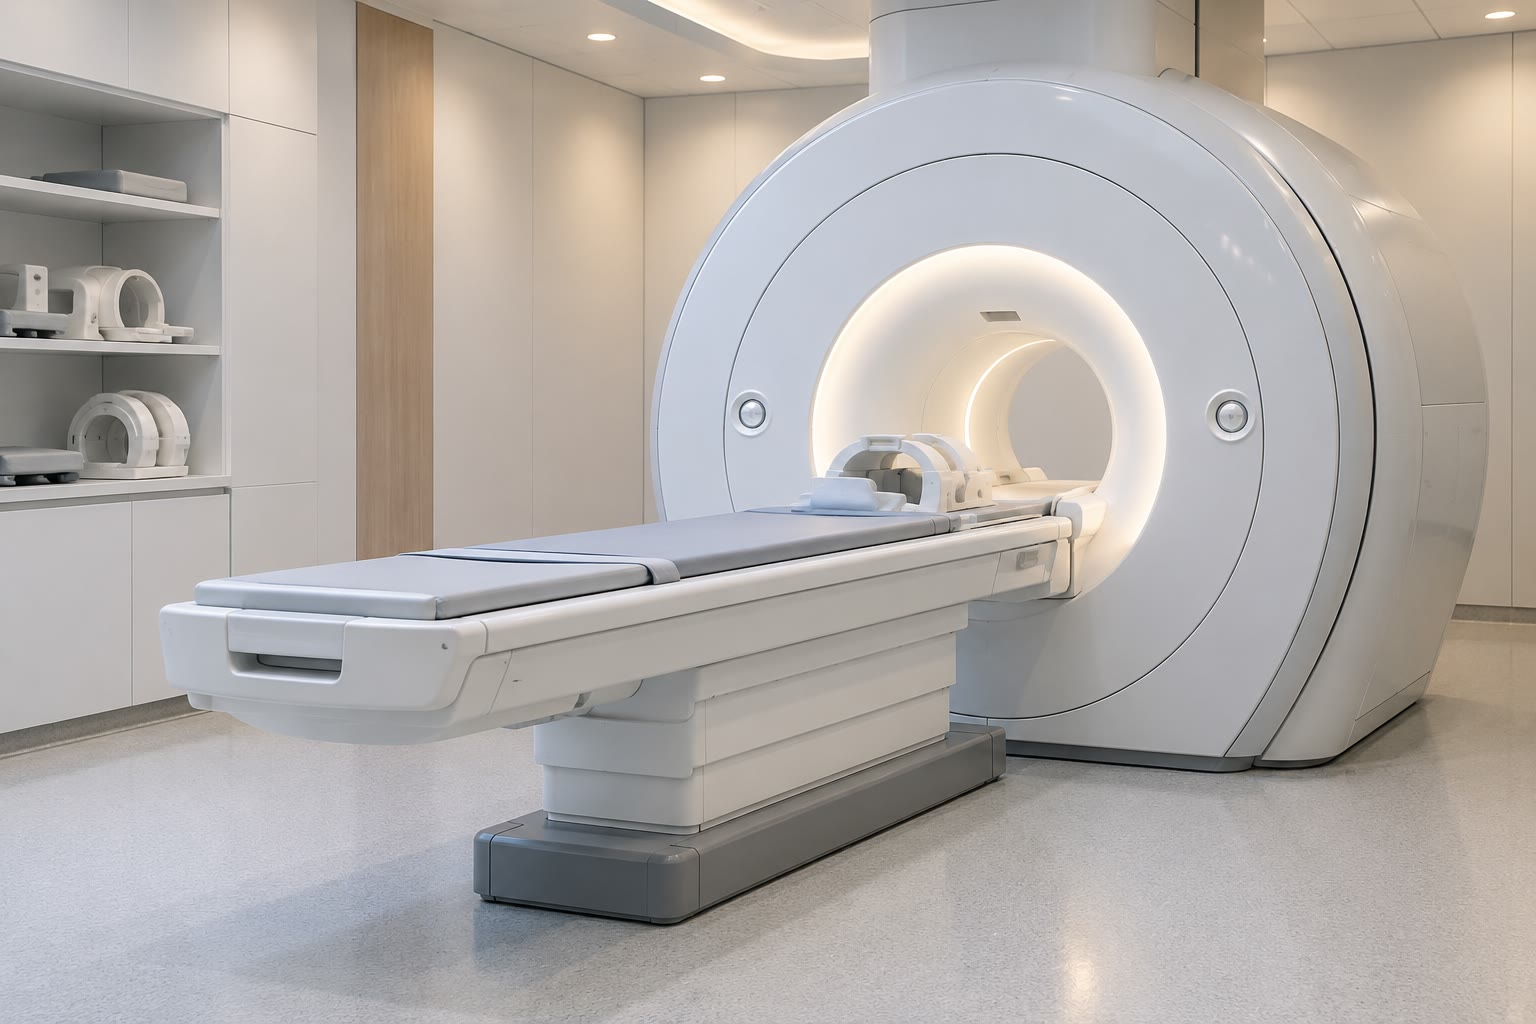
\includegraphics[width=0.52\linewidth]{images/book4/ai/b3-08-mri.jpg}\hspace{0.8em}%
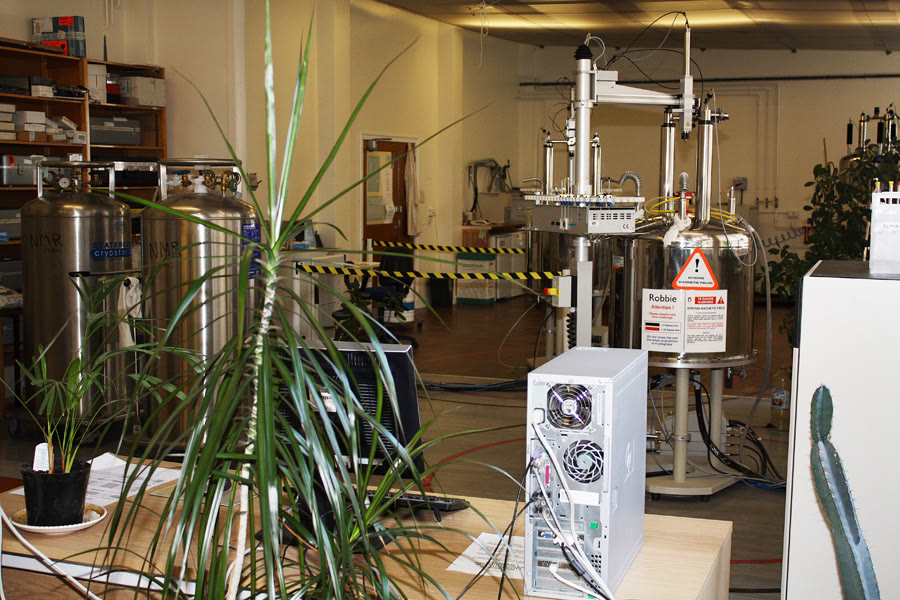
\includegraphics[width=0.4\linewidth]{images/book4/nmr-lab.jpg}

{\small Left: a hospital MRI scanner. Right: an NMR laboratory; each
superconducting magnet stands in its cryostat, refilled with liquid helium
and liquid nitrogen from the dewars on the left. Photograph Shandchem,
CC BY 2.0.}
\end{omfigure}

\section{Nuclear spins in a magnetic field}

\begin{definition}[Nuclear spin quantum number, gyromagnetic ratio]\label{def:b3:advanced-nmr:nuclear-spin}
A nucleus has a spin angular momentum of quantum number $I$, its
\emph{nuclear spin quantum number}\index{nuclear spin quantum number} ($I = 0$
for \ce{^{12}C}, \ce{^{16}O}; $\frac12$ for \ce{^1H}, \ce{^{13}C}, \ce{^{15}N}, \ce{^{19}F},
\ce{^{31}P}; 1 for \ce{^2H}, \ce{^{14}N}), and a magnetic moment $\boldsymbol\mu = \gamma\hat{\mathbf
I}$ proportional to it; $\gamma$ is the \emph{gyromagnetic ratio}\index{gyromagnetic ratio}.
Along a field $B_0$ (axis $z$), $\hat I_z$ takes the values $m_I\hbar$,
$m_I = -I, \dots, I$.
\end{definition}

\begin{proposition}[Zeeman levels]\label{prop:b3:advanced-nmr:zeeman}
In a field $B_0$ the levels are $E_m = -m_I\gamma\hbar B_0$; the transitions $\Delta m_I = \pm1$
absorb at the frequency
\[
\nu_0 = \frac{\gamma B_0}{2\pi}.
\]
\end{proposition}

\begin{proof}
$E = -\boldsymbol\mu\cdot\mathbf B = -\gamma B_0\hat I_z$, of \omterm{def:b3:quantum-model-systems:operator}{eigenvalues} $-\gamma B_0m_I\hbar$. Adjacent
levels differ by $\gamma\hbar B_0 = h\nu_0$.
\end{proof}

\begin{definition}[Larmor frequency]\label{def:b3:advanced-nmr:larmor}
$\nu_0 = \gamma B_0/2\pi$ is the \emph{Larmor frequency}\index{Larmor frequency} of the
nucleus: the frequency of the resonance, and also the frequency at which its
magnetic moment precesses about the field.
\end{definition}

\begin{example}[The common nuclei]\label{ex:b3:advanced-nmr:nuclei}
% ledger: const:gammaP, nuc:C13.mu, nuc:F19.mu, nuc:P31.mu, nuc:N15.mu, const:muN
For a spin-$\frac12$ nucleus of moment $\mu$, $\gamma/2\pi = \mu/(Ih) = 2\mu/h$. With the
measured moments: \ce{^1H} \qty{42.58}{MHz/T}, \ce{^{19}F} \qty{40.08}{MHz/T}, \ce{^{31}P}
\qty{17.25}{MHz/T}, \ce{^{13}C} \qty{10.71}{MHz/T}, \ce{^{15}N} \qty{-4.32}{MHz/T}. A
``\qty{400}{MHz} spectrometer'' has $B_0 = \qty{9.4}{T}$: its protons resonate at
\qty{400.2}{MHz}, its carbons at \qty{100.7}{MHz}.
\end{example}

\begin{proposition}[A tiny population difference]\label{prop:b3:advanced-nmr:populations}
For spin $\frac12$ at temperature $T$, the excess of nuclei in the lower level is
\[
\frac{N_\alpha - N_\beta}{N} \approx \frac{\gamma\hbar B_0}{2kT}.
\]
\end{proposition}

\begin{proof}
$N_\beta/N_\alpha = \eu^{-\Delta E/kT} \approx 1 - \Delta E/kT$ since $\Delta E \ll kT$; so
$(N_\alpha - N_\beta)/(N_\alpha + N_\beta) \approx \Delta E/2kT$, with $\Delta E = \gamma\hbar B_0$.
\end{proof}

For protons at \qty{9.4}{T} and \qty{300}{K} the excess is \num{3.2e-5}: only
three nuclei in a hundred thousand contribute. Since both the excess and the
voltage induced in the coil grow with $\gamma$ and $B_0$, the signal grows
roughly as $\gamma^3B_0^2$: the reason for ever stronger magnets, and for the low
sensitivity of nuclei with small $\gamma$ and low natural abundance such as
\ce{^{13}C}.

\section{Pulses and the free induction decay}

\begin{definition}[Net magnetisation, rotating frame]\label{def:b3:advanced-nmr:magnetisation}
The \emph{net magnetisation}\index{net magnetisation} $\mathbf M$ of a sample is the
sum of its nuclear magnetic moments per unit volume; at equilibrium it is
$M_0$ along $\mathbf B_0$. The \emph{rotating frame}\index{rotating frame} is a set
of axes $x'$, $y'$, $z$ turning about $z$ at the frequency of the radio waves
applied; in it the precession at $\nu_0$ is seen slowed to the offset $\nu_0 -
\nu_{\mathrm{rf}}$.
\end{definition}

\begin{proposition}[Precession]\label{prop:b3:advanced-nmr:precession}
A magnetisation in a field obeys $\dd\mathbf M/\dd t = \gamma\,\mathbf M\times\mathbf B$; in a
static field $B_0\mathbf e_z$, its transverse component turns about $z$ at the angular
frequency $\omega_0 = \gamma B_0$ while $M_z$ stays constant.
\end{proposition}

\begin{proof}[Partial proof]
The equation is the classical torque equation for a magnetic moment carrying
angular momentum, admitted from physics. With $\mathbf B = B_0\mathbf e_z$: $\dot M_x = \gamma
B_0M_y$, $\dot M_y = -\gamma B_0M_x$, $\dot M_z = 0$, whose solution is $M_x + \iu M_y \propto
\eu^{-\iu\gamma B_0t}$: a rotation at $\omega_0$ (clockwise seen from $+z$ for $\gamma > 0$).
\end{proof}

\begin{definition}[Radiofrequency pulse, flip angle]\label{def:b3:advanced-nmr:pulse}
A \emph{radiofrequency pulse}\index{radiofrequency pulse} is a short burst of
radio waves at $\nu_{\mathrm{rf}} \approx \nu_0$, whose magnetic field $B_1$, fixed in the
\omterm{def:b3:advanced-nmr:magnetisation}{rotating frame} along $x'$, turns $\mathbf M$ about $x'$. The angle turned is the
\emph{flip angle}\index{flip angle} $\theta = \gamma B_1t_p$ for a pulse of duration
$t_p$: a $90^\circ$ pulse brings $\mathbf M$ into the $x'y'$ plane, a $180^\circ$ pulse inverts
it.
\end{definition}

\begin{omfigure}
\tdplotsetmaincoords{70}{120}
\begin{tikzpicture}[tdplot_main_coords, font=\small, >=Stealth]
  \begin{scope}
    \draw[->, gray] (0,0,0) -- (1.8,0,0) node[anchor=north east] {$x'$};
    \draw[->, gray] (0,0,0) -- (0,1.8,0) node[anchor=north west] {$y'$};
    \draw[->, gray] (0,0,0) -- (0,0,1.8) node[anchor=south] {$z$, $\mathbf B_0$};
    \draw[->, omThm, very thick] (0,0,0) -- (0,0,1.4) node[anchor=west] {$\mathbf M$};
    \node[anchor=north] at (0,0,-0.9) {equilibrium};
  \end{scope}
  \begin{scope}[shift={(0,4.6,0)}]
    \draw[->, gray] (0,0,0) -- (1.8,0,0) node[anchor=north east] {$x'$};
    \draw[->, gray] (0,0,0) -- (0,1.8,0) node[anchor=north west] {$y'$};
    \draw[->, gray] (0,0,0) -- (0,0,1.8) node[anchor=south] {$z$};
    \draw[->, omDef, thick] (0,0,0) -- (1.2,0,0) node[anchor=south east, xshift=-2pt] {$\mathbf B_1$};
    \draw[->, omThm, very thick] (0,0,0) -- (0,1.4,0) node[anchor=south west] {$\mathbf M$};
    \node[anchor=north] at (0,0,-0.9) {after a $90^\circ_{x'}$ pulse};
  \end{scope}
  \begin{scope}[shift={(0,9.2,0)}]
    \draw[->, gray] (0,0,0) -- (1.8,0,0) node[anchor=north east] {$x'$};
    \draw[->, gray] (0,0,0) -- (0,1.8,0) node[anchor=north west] {$y'$};
    \draw[->, gray] (0,0,0) -- (0,0,1.8) node[anchor=south] {$z$};
    \draw[->, omThm, very thick] (0,0,0) -- (0,0,-1.4) node[anchor=west] {$\mathbf M$};
    \node[anchor=north] at (0,0,-1.6) {after a $180^\circ_{x'}$ pulse};
  \end{scope}
\end{tikzpicture}

{\small The magnetisation in the \omterm{def:b3:advanced-nmr:magnetisation}{rotating frame}. A $90^\circ$ pulse about $x'$
turns $\mathbf M$ from $z$ to $y'$ (with $\gamma > 0$ the rotation follows the
left-hand rule about $\mathbf B_1$, the usual convention); a $180^\circ$ pulse
inverts it.}
\end{omfigure}

\begin{definition}[Free induction decay]\label{def:b3:advanced-nmr:fid}
After a $90^\circ$ pulse, the transverse magnetisation precesses at the \omterm{def:b3:advanced-nmr:larmor}{Larmor
frequency} and induces an oscillating voltage in the coil around the sample,
which dies away as the magnetisation relaxes: the \emph{free induction
decay}\index{free induction decay} (FID).
\end{definition}

\begin{theorem}[From the FID to the spectrum]\label{thm:b3:advanced-nmr:lorentzian}
The Fourier transform of a decaying oscillation $\eu^{-t/T_2}\cos(2\pi\nu t)$ ($t \ge 0$) is,
near $\nu$, a Lorentzian line of full width at half maximum $1/(\pi T_2)$.
\end{theorem}

\begin{proof}
Write the signal $\eu^{-t/T_2}\eu^{2\pi\iu\nu t}$ and integrate:
$\int_0^\infty\eu^{-t/T_2}\eu^{2\pi\iu(\nu - f)t}\dd t = \frac{1}{1/T_2 - 2\pi\iu(\nu - f)}$, whose real
part is $\frac{T_2}{1 + 4\pi^2T_2^2(f - \nu)^2}$. It is maximal at $f = \nu$ and falls to
half when $2\pi T_2|f - \nu| = 1$, i.e. at $f - \nu = \pm1/(2\pi T_2)$: a full width
$1/(\pi T_2)$.
\end{proof}

\begin{omfigure}
\begin{tikzpicture}
\begin{axis}[name=fid, width=0.5\linewidth, height=4.6cm, xmin=0, xmax=0.4,
  ymin=-2.1, ymax=2.1, axis lines=left, xlabel={$t$ / s}, ylabel={signal},
  ytick=\empty, scaled x ticks=false, xticklabel style={/pgf/number format/fixed},
  tick label style={font=\small}, label style={font=\small}, title={\small FID}]
\addplot[omDef] table[x=t, y=s] {figdata/out/bachelor-3-nmr-fid.dat};
\addplot[gray, dashed, domain=0:0.4, samples=60] {2*exp(-x/0.1)};
\end{axis}
\begin{axis}[at={(fid.east)}, anchor=west, xshift=1.2cm, width=0.45\linewidth,
  height=4.6cm, xmin=0, xmax=350, ymin=-0.1, ymax=1.1, axis x line=bottom,
  axis y line=none, xlabel={offset / Hz}, tick label style={font=\small},
  label style={font=\small}, title={\small spectrum (Fourier transform)}]
\addplot[omThm, thick] table[x=f, y=I] {figdata/out/bachelor-3-nmr-fid-spectrum.dat};
\end{axis}
\end{tikzpicture}

{\small Left: the FID of two lines (offsets 100 and \qty{250}{Hz}, $T_2 = \qty{0.10}{s}$),
beating as the two frequencies interfere inside an exponential envelope
(dashed). Right: its Fourier transform, two Lorentzian lines \qty{3.2}{Hz} wide.}
\end{omfigure}

\begin{proposition}[Signal averaging]\label{prop:b3:advanced-nmr:averaging}
Adding $N$ FIDs multiplies the signal by $N$ and the random noise by $\sqrt N$:
the signal-to-noise ratio grows as $\sqrt N$.
\end{proposition}

\begin{proof}
The signal adds coherently. The noise of independent acquisitions has zero
mean and variance $\sigma^2$ each; the variance of a sum of $N$ independent terms is
$N\sigma^2$ (the propagation law of the Year 2 volume), so its standard deviation
is $\sqrt N\sigma$.
\end{proof}

DEPT, which sorts ${}^{13}$C signals by the number of attached hydrogens,
applies a sequence of pulses to both protons and carbons separated by
delays of $1/2J$: the large proton magnetisation is transferred to the carbon
through the one-bond coupling, which multiplies the carbon signal by about
$\gamma_H/\gamma_C \approx 4$, and the final proton pulse angle weights CH, \ce{CH2} and
\ce{CH3} differently. The same idea --- moving magnetisation between nuclei
through their couplings --- underlies the two-dimensional experiments below.

\section{Relaxation}

\begin{definition}[Longitudinal and transverse relaxation times]\label{def:b3:advanced-nmr:relaxation}
The return of $M_z$ to $M_0$ after a perturbation is exponential, with the
\emph{longitudinal relaxation time}\index{longitudinal relaxation time} $T_1$
(spin--lattice relaxation: energy given to the surroundings). The decay of
the transverse magnetisation to zero is exponential with the
\emph{transverse relaxation time}\index{transverse relaxation time} $T_2 \le T_1$
(spin--spin relaxation: loss of phase coherence between spins).
\end{definition}

\begin{proposition}[Inversion recovery]\label{prop:b3:advanced-nmr:inversion-recovery}
After a $180^\circ$ pulse, $M_z(t) = M_0(1 - 2\eu^{-t/T_1})$; it passes through zero at
$t_{\mathrm{null}} = T_1\ln2$.
\end{proposition}

\begin{proof}
The relaxation equation $\dd M_z/\dd t = (M_0 - M_z)/T_1$ with $M_z(0) = -M_0$ has the
solution $M_0 - 2M_0\eu^{-t/T_1}$, which vanishes when $\eu^{-t/T_1} = \frac12$.
\end{proof}

\begin{method}[Measuring $T_1$ and setting a quantitative recycle delay]\label{met:b3:advanced-nmr:t1}
\begin{enumerate}
  \item Run the sequence $180^\circ$--$\tau$--$90^\circ$--acquire for a series of delays
        $\tau$, waiting at least $5T_1$ between scans.
  \item Fit each signal to $M_0(1 - 2\eu^{-\tau/T_1})$, or read the null: $T_1 =
        t_{\mathrm{null}}/\ln2$.
  \item For quantitative integration with $90^\circ$ pulses, wait at least $5T_1$ of the
        slowest nucleus between scans: then $\eu^{-5} < 1\,\%$ of the magnetisation is
        missing.
\end{enumerate}
\end{method}

\begin{omfigure}
\begin{tikzpicture}
\begin{axis}[width=0.62\linewidth, height=5cm, xmin=0, xmax=10, ymin=-1.1, ymax=1.15,
  axis lines=left, xlabel={$t$ / s}, ylabel={$M/M_0$}, legend cell align=left,
  legend style={font=\small, draw=none, at={(0.97,0.05)}, anchor=south east},
  tick label style={font=\small}, label style={font=\small}]
\addplot[omDef, thick] table[x=t, y=mz] {figdata/out/bachelor-3-nmr-relaxation.dat};
\addlegendentry{$M_z$ after $180^\circ$ ($T_1 = \qty{2.0}{s}$)}
\addplot[omThm, thick, dashed] table[x=t, y=mxy] {figdata/out/bachelor-3-nmr-relaxation.dat};
\addlegendentry{$M_{xy}$ after $90^\circ$ ($T_2 = \qty{0.5}{s}$)}
\addplot[gray, dotted, domain=0:10] {0};
\addplot[only marks, mark=*, mark size=1.5pt, black] coordinates {(1.386,0)};
\node[font=\small, anchor=north west] at (axis cs:1.5,-0.04) {$T_1\ln2$};
\end{axis}
\end{tikzpicture}

{\small Relaxation (model values). The inverted longitudinal magnetisation
recovers through zero at $T_1\ln2$; the transverse magnetisation decays
faster, with $T_2$.}
\end{omfigure}

\begin{definition}[Spin echo]\label{def:b3:advanced-nmr:echo}
In the sequence $90^\circ$--$\tau$--$180^\circ$--$\tau$, spins that drifted apart in phase
because of field inhomogeneities are refocused at time $2\tau$, producing a
\emph{spin echo}\index{spin echo}; its amplitude decays with the true $T_2$, free of
the inhomogeneity of the magnet.
\end{definition}

\begin{definition}[Nuclear Overhauser effect]\label{def:b3:advanced-nmr:noe}
Saturating or perturbing one spin changes, through their dipolar
relaxation, the intensity of the signal of another spin close in space:
the \emph{nuclear Overhauser effect}\index{nuclear Overhauser effect} (NOE).
Its build-up rate is proportional to $r^{-6}$, so it is seen only between
nuclei less than about \qty{0.5}{nm} apart, whether bonded or not.
\end{definition}

\section{Two-dimensional NMR}

\begin{definition}[Two-dimensional spectrum, cross peak, diagonal peak]\label{def:b3:advanced-nmr:two-d}
A \emph{two-dimensional spectrum}\index{two-dimensional spectrum} is recorded by
repeating a pulse sequence with an incremented delay $t_1$ before the
acquisition time $t_2$; a double Fourier transform gives a map of intensity
against two frequencies. A \emph{cross peak}\index{cross peak} at $(\delta_1,
\delta_2)$ shows that the nuclei at $\delta_1$ and $\delta_2$ are connected (by a coupling or
by proximity); a \emph{diagonal peak}\index{diagonal peak} at $(\delta, \delta)$ belongs to
a single nucleus.
\end{definition}

\begin{definition}[COSY, HSQC, HMBC, NOESY]\label{def:b3:advanced-nmr:experiments}
\emph{COSY}\index{COSY} (correlation spectroscopy) correlates protons coupled
to each other, usually through three bonds (H--C--C--H). \emph{HSQC}\index{HSQC}
(heteronuclear single-quantum coherence) correlates each carbon with the
protons directly bonded to it. \emph{HMBC}\index{HMBC} (heteronuclear
multiple-bond correlation) correlates carbons with protons two or three bonds
away, across quaternary carbons and heteroatoms. \emph{NOESY}\index{NOESY}
correlates protons close in space through the \omterm{def:b3:advanced-nmr:noe}{nuclear Overhauser effect}.
\end{definition}

\begin{omfigure}
\begin{tikzpicture}[font=\small]
  \foreach \y/\name in {3.2/{one pulse}, 2.0/{inversion recovery}, 0.8/{spin echo}, -0.4/{COSY}}{
    \draw (0,\y) -- (9.3,\y); \node[anchor=east] at (-0.1,\y+0.25) {\name};}
  % one pulse
  \fill[black] (0.4,3.2) rectangle (0.6,3.75);
  \draw[omDef, domain=0:3.5, samples=120] plot (0.7+\x, {3.2+0.4*exp(-\x/1.2)*sin(\x*500)});
  % inversion recovery
  \fill[black] (0.4,2.0) rectangle (0.8,2.55); \node[font=\scriptsize] at (0.6,2.7) {180};
  \draw[<->] (0.85,1.85) -- (2.4,1.85) node[midway, below, font=\scriptsize] {$\tau$};
  \fill[black] (2.45,2.0) rectangle (2.65,2.55); \node[font=\scriptsize] at (2.55,2.7) {90};
  \draw[omDef, domain=0:3.0, samples=120] plot (2.75+\x, {2.0+0.4*exp(-\x/1.0)*sin(\x*500)});
  % spin echo
  \fill[black] (0.4,0.8) rectangle (0.6,1.35); \node[font=\scriptsize] at (0.5,1.5) {90};
  \draw[<->] (0.65,0.65) -- (2.4,0.65) node[midway, below, font=\scriptsize] {$\tau$};
  \fill[black] (2.45,0.8) rectangle (2.85,1.35); \node[font=\scriptsize] at (2.65,1.5) {180};
  \draw[<->] (2.9,0.65) -- (4.65,0.65) node[midway, below, font=\scriptsize] {$\tau$};
  \draw[omDef, domain=-1.2:2.5, samples=150] plot (4.65+\x, {0.8+0.35*exp(-abs(\x)/0.35)*cos(\x*700)});
  % COSY
  \fill[black] (0.4,-0.4) rectangle (0.6,0.15); \node[font=\scriptsize] at (0.5,0.3) {90};
  \draw[<->] (0.65,-0.55) -- (2.4,-0.55) node[midway, below, font=\scriptsize] {$t_1$ (incremented)};
  \fill[black] (2.45,-0.4) rectangle (2.65,0.15); \node[font=\scriptsize] at (2.55,0.3) {90};
  \draw[omDef, domain=0:3.0, samples=120] plot (2.75+\x, {-0.4+0.4*exp(-\x/1.0)*sin(\x*500)});
  \node[font=\scriptsize, anchor=west] at (5.9,-0.2) {acquire ($t_2$)};
\end{tikzpicture}

{\small Pulse sequences (time to the right; filled boxes: pulses, labelled
with their \omterm{def:b3:advanced-nmr:pulse}{flip angles} in degrees; blue: the recorded signal). The \omterm{def:b3:advanced-nmr:echo}{spin echo}
peaks at $2\tau$ after the first pulse.}
\end{omfigure}

\begin{method}[Solving a structure with two-dimensional spectra]\label{met:b3:advanced-nmr:solve-2d}
\begin{enumerate}
  \item From the formula, the ${}^1$H integrals and the ${}^{13}$C/DEPT spectrum, list
        the CH, \ce{CH2}, \ce{CH3} and quaternary carbons.
  \item \omterm{def:b3:advanced-nmr:experiments}{HSQC}: attach each proton signal to its carbon.
  \item \omterm{def:b3:advanced-nmr:experiments}{COSY}: join the protonated carbons into spin systems (chains of
        neighbours).
  \item \omterm{def:b3:advanced-nmr:experiments}{HMBC}: join the spin systems across quaternary carbons, carbonyls and
        heteroatoms, where \omterm{def:b3:advanced-nmr:experiments}{COSY} is silent.
  \item \omterm{def:b3:advanced-nmr:experiments}{NOESY}: fix relative configurations and conformations from
        through-space contacts.
  \item Check every signal against the proposed structure.
\end{enumerate}
\end{method}

\begin{omfigure}
\begin{tikzpicture}
\begin{axis}[name=cosy, width=0.47\linewidth, height=0.47\linewidth, x dir=reverse,
  y dir=reverse, xmin=0.5, xmax=4.6, ymin=0.5, ymax=4.6, axis lines=box,
  xlabel={$\delta_{\mathrm H}$ / ppm}, ylabel={$\delta_{\mathrm H}$ / ppm},
  tick label style={font=\small}, label style={font=\small}, title={\small COSY}]
\addplot[gray, dotted, domain=0.5:4.6] {x};
\addplot[only marks, mark=*, mark size=2.2pt, black] table[x=h1, y=h2] {figdata/out/bachelor-3-nmr-2d-cosy-diag.dat};
\addplot[only marks, mark=*, mark size=2.2pt, omThm] table[x=h1, y=h2] {figdata/out/bachelor-3-nmr-2d-cosy-cross.dat};
\end{axis}
\begin{axis}[at={(cosy.east)}, anchor=west, xshift=1.3cm, width=0.47\linewidth,
  height=0.47\linewidth, x dir=reverse, y dir=reverse, xmin=0.5, xmax=4.6,
  ymin=0, ymax=185, axis lines=box, xlabel={$\delta_{\mathrm H}$ / ppm},
  ylabel={$\delta_{\mathrm C}$ / ppm}, tick label style={font=\small},
  label style={font=\small}, title={\small HSQC (blue) and HMBC (red)}]
\addplot[only marks, mark=square*, mark size=2.2pt, omDef] table[x=h, y=c] {figdata/out/bachelor-3-nmr-2d-hsqc.dat};
\addplot[only marks, mark=o, mark size=2.6pt, omThm, thick] table[x=h, y=c] {figdata/out/bachelor-3-nmr-2d-hmbc.dat};
\end{axis}
\end{tikzpicture}

{\small Two-dimensional spectra of ethyl butanoate, \ce{CH3CH2CH2COOCH2CH3},
drawn at its measured shifts. \omterm{def:b3:advanced-nmr:experiments}{COSY}: black, \omterm{def:b3:advanced-nmr:two-d}{diagonal peaks}; red, \omterm{def:b3:advanced-nmr:two-d}{cross peaks}
between protons on neighbouring carbons --- two spin systems, ethyl and
propyl, with no \omterm{def:b3:advanced-nmr:two-d}{cross peak} across the ester oxygen. Right: \omterm{def:b3:advanced-nmr:experiments}{HSQC} peaks
(squares) join each proton to its carbon; \omterm{def:b3:advanced-nmr:experiments}{HMBC} peaks (circles) show the OCH$_2$
protons (\qty{4.13}{ppm}) and the CH$_2$C=O protons (\qty{2.28}{ppm}) both reaching the
carbonyl carbon at \qty{173.6}{ppm}.}
\end{omfigure}

\section{Other nuclei and dynamics}

Fluorine-19 and phosphorus-31, spin $\frac12$, 100\,\% abundant and with large
$\gamma$, are almost as easy to observe as protons; their wide ranges of shifts make
them precise probes of their environment (drugs, phosphates, ligands such as
phosphines in \cref{ch:b3:organometallic-bonding}). Nitrogen-15 is rare and
weak, and is usually observed indirectly through the protons bonded to it.
Coupling between different nuclei is removed by decoupling, as for ${}^{13}$C in
the Year 2 volume.

\begin{definition}[Coalescence temperature]\label{def:b3:advanced-nmr:coalescence}
When a nucleus exchanges between two environments of shifts separated by
$\Delta\nu$ (in hertz), its two lines broaden as the exchange speeds up and merge
into one at the \emph{coalescence temperature}\index{coalescence temperature}
$T_c$.
\end{definition}

\begin{proposition}[Rate at coalescence]\label{prop:b3:advanced-nmr:coalescence}
For two equally populated sites without coupling, the exchange rate constant at
coalescence is $k_c = \pi\Delta\nu/\sqrt2$.
\end{proposition}
\admitted

The derivation, from the Bloch equations with exchange, is treated in more
advanced courses. With the Eyring equation (\cref{ch:b3:rate-theories}) the rate
gives the barrier: dynamic NMR measures rotations about amide bonds, ring
flips and ligand exchanges with barriers of 40 to \qty{100}{kJ/mol}.

\begin{example}[An MRI image]\label{ex:b3:advanced-nmr:mri}
In magnetic resonance imaging a field gradient makes the \omterm{def:b3:advanced-nmr:larmor}{Larmor frequency} of
the water protons depend on position, so that the Fourier transform of the
signal is a map of where they are. Contrast comes from relaxation: the
repetition time and echo delays are chosen to weight the image by $T_1$ or by
$T_2$, which differ between tissues; contrast agents containing gadolinium
shorten the $T_1$ of nearby water (\cref{ch:b3:bioinorganic}).
\end{example}

\begin{inthelab}[Preparing a spectrometer]
The sample, dissolved in a deuterated solvent, is lowered into the probe.
The spectrometer locks on the deuterium signal to compensate the slow drift of
the field; the probe is tuned and matched to the frequency of each nucleus;
the field is made homogeneous over the sample by adjusting the shim coils
until the lines are narrow. The magnet's field is permanent: steel tools,
credit cards and pacemakers are kept outside the marked safety line.
\end{inthelab}

\begin{history}[From resonance to two dimensions]
Felix Bloch and Edward Purcell detected nuclear magnetic resonance in bulk
matter in 1946 (Nobel Prize in Physics, 1952). Richard Ernst introduced pulsed
Fourier-transform NMR in 1966 and, following an idea of Jean Jeener,
two-dimensional spectroscopy in the 1970s (Nobel Prize in Chemistry, 1991).
\end{history}

\section{Exercises}

\begin{exercise}[$\star$]\label{exo:b3:advanced-nmr:1}
% ledger: const:gammaP, nuc:C13.mu, nuc:F19.mu
Compute the Larmor frequencies of \ce{^1H}, \ce{^{13}C} and \ce{^{19}F} at \qty{14.1}{T}
($\gamma/2\pi = 42.58$, 10.71 and \qty{40.08}{MHz/T}).
\end{exercise}

\begin{exercise}[$\star$]\label{exo:b3:advanced-nmr:2}
Compute the relative excess of protons in the lower level at \qty{9.4}{T} and
\qty{300}{K}. By how much does it change at \qty{4}{K}?
\end{exercise}

\begin{exercise}[$\star$]\label{exo:b3:advanced-nmr:3}
A $90^\circ$ pulse lasts \qty{10}{\micro s} for protons. What is $\gamma B_1/2\pi$? How long is a
$180^\circ$ pulse, and what does a \qty{5}{\micro s} pulse do?
\end{exercise}

\begin{exercise}[$\star$]\label{exo:b3:advanced-nmr:4}
A line is \qty{3.2}{Hz} wide at half height. What is $T_2$ (assuming a perfectly
homogeneous field)?
\end{exercise}

\begin{exercise}[$\star\star$]\label{exo:b3:advanced-nmr:5}
% ledger: iso:C13
Using signal $\propto\gamma^3$ per nucleus and the 1.1\,\% natural abundance of
\ce{^{13}C}, compare the sensitivity of ${}^{13}$C and ${}^1$H NMR. How many more scans
does a ${}^{13}$C spectrum need for the same signal-to-noise ratio?
\end{exercise}

\begin{exercise}[$\star\star$]\label{exo:b3:advanced-nmr:6}
In an inversion-recovery experiment the signal of a carbon vanishes at
$\tau = \qty{1.39}{s}$. Find $T_1$ and the recycle delay for quantitative work.
\end{exercise}

\begin{exercise}[$\star\star$]\label{exo:b3:advanced-nmr:7}
In the \omterm{def:b3:advanced-nmr:experiments}{COSY} spectrum of butanone, \ce{CH3COCH2CH3}, which \omterm{def:b3:advanced-nmr:two-d}{cross peaks} appear?
Which carbons show \omterm{def:b3:advanced-nmr:experiments}{HMBC} peaks from the singlet methyl protons?
\end{exercise}

\begin{exercise}[$\star\star$]\label{exo:b3:advanced-nmr:8}
Two methyl signals of an amide, \qty{50}{Hz} apart at low temperature, coalesce at
\qty{330}{K}. Compute the exchange rate at coalescence and the Gibbs energy of
activation with $\Delta G^\ddagger = RT_c\ln(k_BT_c/hk_c)$.
\end{exercise}

\begin{exercise}[$\star\star$]\label{exo:b3:advanced-nmr:9}
An NOE between protons H$_a$ and H$_b$ is four times stronger than between H$_a$ and
H$_c$, at \qty{0.30}{nm}. Estimate the H$_a$--H$_b$ distance.
\end{exercise}

\begin{exercise}[$\star\star\star$]\label{exo:b3:advanced-nmr:10}
Show, by solving $\dd\mathbf M/\dd t = \gamma\mathbf M\times\mathbf B_1$ in the \omterm{def:b3:advanced-nmr:magnetisation}{rotating frame}
with $\mathbf B_1$ along $x'$, that a pulse rotates $\mathbf M$ by $\gamma B_1t_p$ about $x'$.
\end{exercise}

\begin{exercise}[$\star\star\star$]\label{exo:b3:advanced-nmr:11}
Explain why the \omterm{def:b3:advanced-nmr:echo}{spin echo} refocuses the dephasing due to an inhomogeneous
field but not that due to random interactions between spins. Which time
constant does the echo amplitude measure?
\end{exercise}

\begin{exercise}[$\star\star\star$]\label{exo:b3:advanced-nmr:12}
Propose the structure of a compound \ce{C4H8O2} whose ${}^1$H spectrum shows a
quartet (2H, 4.12 ppm), a singlet (3H, 2.05 ppm) and a triplet (3H,
1.26 ppm), and whose \omterm{def:b3:advanced-nmr:experiments}{HMBC} spectrum correlates the quartet protons with a
carbon at 171 ppm (data of the exercise). Which other ester of the same
formula would give a different \omterm{def:b3:advanced-nmr:experiments}{HMBC} pattern, and how?
\end{exercise}

\section{Problem: The Pineapple Ester in Two Dimensions}

\begin{problem}[{Weekend problem --- ethyl butanoate solved again, from
two-dimensional spectra: spin systems from COSY, carbons from HSQC, the
ester linkage from HMBC, and the delay needed for a quantitative carbon
spectrum}]
\label{pb:b3:advanced-nmr:1}
% ledger: nmr:ethylbutanoate-OCH2, nmr:ethylbutanoate-CH2CO, nmr:ethylbutanoate-CH2, nmr:ethylbutanoate-OCH2CH3, nmr:ethylbutanoate-CH3, c13:ethylbutanoate.CO, c13:ethylbutanoate.OCH2, c13:ethylbutanoate.CH2CO, c13:ethylbutanoate.CH2, c13:ethylbutanoate.OCH2CH3, c13:ethylbutanoate.CH3
An ester \ce{C6H12O2} from the aroma of pineapple shows ${}^1$H signals at 4.13 (2H,
q), 2.28 (2H, t), 1.66 (2H, m), 1.25 (3H, t) and 0.95 ppm (3H, t), and ${}^{13}$C signals
at 173.6, 60.1, 36.3, 18.6, 14.3 and 13.7 ppm, recorded at \qty{9.4}{T}. Its 2D
spectra are those of the figure of section 4. Data of the problem: the $T_1$
values of the carbons are about \qty{20}{s} for the carbonyl and 2 to \qty{6}{s} for the
others.

\medskip\noindent\textbf{Part I --- One dimension.}
\begin{enumerate}
  \item Compute the degree of unsaturation of \ce{C6H12O2}.
  \item Which ${}^{13}$C signal is the carbonyl? Which is the carbon bonded to oxygen?
  \item How many protonated carbons are there? What would DEPT-135 show?
  \item At \qty{9.4}{T}, what are the Larmor frequencies of ${}^1$H and ${}^{13}$C?
  \item The coupling of the quartet is \qty{7.2}{Hz}. How wide, in ppm, is the
        quartet at \qty{400}{MHz}?
  \item Why can the 1D spectra alone leave the order of the fragments open?
\end{enumerate}

\medskip\noindent\textbf{Part II --- \omterm{def:b3:advanced-nmr:experiments}{COSY}.}
\begin{enumerate}[resume]
  \item List the \omterm{def:b3:advanced-nmr:two-d}{cross peaks} of the \omterm{def:b3:advanced-nmr:experiments}{COSY} map.
  \item Deduce the two spin systems.
  \item Why is there no \omterm{def:b3:advanced-nmr:two-d}{cross peak} between 4.13 and 2.28 ppm?
  \item Which proton signal is coupled to two others? Explain its multiplicity.
  \item What would a \omterm{def:b3:advanced-nmr:two-d}{cross peak} between 0.95 and 1.25 ppm have meant?
  \item Draw the two fragments.
\end{enumerate}

\medskip\noindent\textbf{Part III --- \omterm{def:b3:advanced-nmr:experiments}{HSQC} and \omterm{def:b3:advanced-nmr:experiments}{HMBC}.}
\begin{enumerate}[resume]
  \item From the \omterm{def:b3:advanced-nmr:experiments}{HSQC}, assign each carbon to its protons.
  \item Which two methyl carbons are distinguished only by the \omterm{def:b3:advanced-nmr:experiments}{HSQC}?
  \item Which \omterm{def:b3:advanced-nmr:experiments}{HMBC} peak links the ethyl fragment to the carbonyl, and through
        how many bonds?
  \item Which \omterm{def:b3:advanced-nmr:experiments}{HMBC} peaks link the propyl fragment to the carbonyl?
  \item Deduce the structure, and exclude its isomer propyl propanoate.
  \item Why are \omterm{def:b3:advanced-nmr:experiments}{HMBC} peaks across four bonds or more usually absent?
\end{enumerate}

\medskip\noindent\textbf{Part IV --- A quantitative carbon spectrum.}
\begin{enumerate}[resume]
  \item Why are the integrals of an ordinary ${}^{13}$C spectrum not proportional to
        the number of carbons?
  \item What fraction of its equilibrium magnetisation does the carbonyl recover
        if scans are repeated every \qty{5}{s} with $90^\circ$ pulses (starting each time
        from zero)?
  \item What fraction after $5T_1$?
  \item Besides relaxation, which effect of proton decoupling distorts carbon
        integrals, and how is it suppressed?
  \item With a delay of $5T_1$, how long do 256 scans take?
  \item State the result: the minimum recycle delay for a quantitative ${}^{13}$C
        spectrum of this ester.
\end{enumerate}
\end{problem}
